\section[Force Model: Net Force and Force Diagrams]{Force Model: Net Force and Force Diagrams\protect{\footnote{See Pages~41-51 of course notes and Force Model Summary.}}}
\label{act6.2.1}

\begin{overview}

\textbf{Overview:} Now that we can represent linear and curved motion with vectors, let's see how vectors are tremendously useful to describe \emph{forces}, as well.

\end{overview}

\noindent\textbf{Phenomenon:} You are going to pull on a metal ring with three ropes attached. A spring is attached to each rope to determine the tension in the rope.

\begin{itemize}
	\item Before you start, make sure each scale is set to zero by twisting the knob.
	\item Work together as a group. No, really: This takes multiple hands!
	\item Attach the ropes with the scales turned so you can read force values in Newtons.
\end{itemize}

\noindent\textbf{Note:} To get the angles to be 130\textdegree{}, trace the ring on a sheet of paper and draw a vertical line pointing down from it. Use a protractor to mark the 130\textdegree{} angles from the vertical line. Line up the ropes along the lines you drew, pull and then note the force scale readings.

\begin{figure}[h!]
	\vspace{-4pt}
	\centering
	\begin{subfigure}[b]{0.45\textwidth}
		\centering
		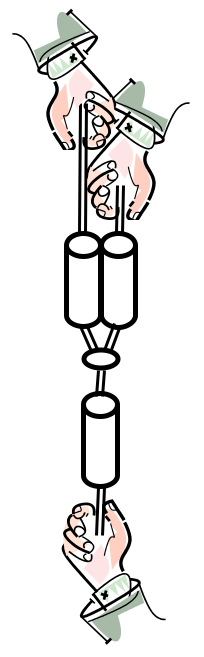
\includegraphics[width=0.25\textwidth]{act621-scenario1}
		\begin{tikzpicture}[thick,scale=0.65, every node/.style={transform shape},background rectangle/.style={fill=white}, show background rectangle]
			% draw object node
			\draw (0,3.5) node[circle,minimum size=12pt,fill,inner sep=1pt]{} node[right=6pt]{Ring};	
			
			% draw and label F1
			\draw[-{Stealth[scale=1.2]}, line width=1pt] (0,3.5) -- (0,5.25) node[right=3pt,align=center] {$\vec{F}_\text{Scale 1 on Ring}$};
			% draw and label F2
			\draw[-{Stealth[scale=1.2]}, line width=1pt] (0,5.25) -- (0,7) node[right=3pt,align=center] {$\vec{F}_\text{Scale 2 on Ring}$};
			
			% draw and label F3
			\draw[-{Stealth[scale=1.2]}, line width=1pt] (0,3.5) -- (0,0) node[right=3pt,align=center] {$\vec{F}_\text{Scale 3 on Ring}$};
		\end{tikzpicture}
		\caption*{\textbf{Scenario 1:} Person~1 and Person~2 pull directly opposite to Person~3 so that the yellow spring scale for the third person reads \unit[30]{N}. Record the values on all three scales.}
	\end{subfigure}
	\hspace{0.05\textwidth}
	\begin{subfigure}[b]{0.45\textwidth}
		\centering
		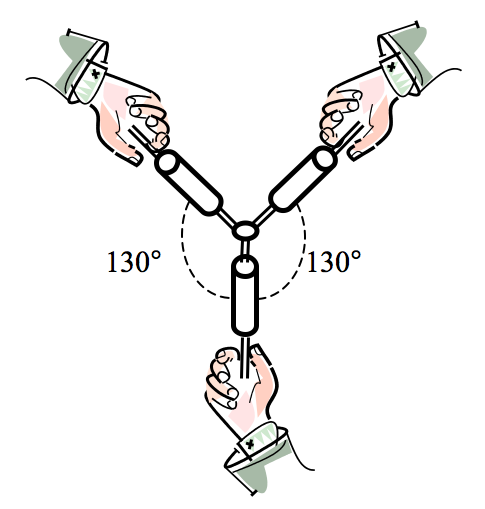
\includegraphics[width=0.5\textwidth]{act621-scenario2}
		\caption*{\textbf{Scenario 2:}  Persons~1 and 2 change the direction they are pulling until their ropes make an angle of about 130\textdegree{} with respect to Person~3. Record the readings of all scales.}
	\end{subfigure}
\end{figure}

\begin{enumerate}
	\item \label{621,1} Use appropriately scaled force vectors from the sheet of paper you've used as a guide, and graphically add the three vectors while preserving their angles on the board. What do you get? Why is that? Draw and label all vector components on your graph.
	\note{\ref{621,1}:}{For scenario 2: when added graphically, the 3 vectors are all arrow to tail and closed .  If they try drawing the net force, they get the tail and arrow (head) at nearly the same place, or net force = 0.  Make sure they see/understand this.  Remind them that they can slide vectors around to add them, preserving their original angles.  This part is to give them practice with force vector addition and concept of net force.  Make sure they label the components; this will help some students understand how the magnitudes of the vertical components for forces 1 \& 2 add to equal magnitude of force 3, and the horizontal components add to zero.
	\\[0.25in]
Encourage proper labeling of all vectors.  For forces this means two subscripts: one showing the object exerting the force, the other the object the force is acting on.  The students will need to refer to pages 8-9 in Course Notes for proper labeling.  
	\\[0.25in]
This part further emphasizes vector addition and concept of net force.  We emphasize how net force is found, either by graphical addition of vectors or by components.  
	\\[0.25in]
Encourage the use of two lines to distinguish the net force from the real forces (although here the net force is zero).  Do not let students skimp on part (d).  You should make sure this comes out clearly in the quick \WC{} discussion just before they start this part.  Have them put their responses on the board.
	}
	\item \label{621,2} A properly labeled and scaled force diagram for the ring is shown for Scenario 1 (on the left, above). \textbf{Note:} Two forces acting on the same object and going in the same direction can be drawn as shown here, or both arrows can have their tails attached to the dot.
	\note{\ref{621,2}:}{Students often get confused with the difference between the force vector (magnitude and direction) and its components.  Help them out here, and with 2) above, by having them draw the force vectors $F_{1}$ on ring and $F_{2}$ on ring to scale for this situation (along with$F_{3}$ on ring).  Then have them identify the components and see why the vertical components of the forces cannot possibly be balanced as the separation of forces 1 and 2 gets closer to 180$^{\circ}$.}	
	Draw a properly labeled and scaled force diagram for the ring: model it as an object with the three forces acting on it, as in Scenario 2. Be sure to use the labeling conventions spelled out on Page~43 of the textbook on any force diagram you make.
\end{enumerate}\begin{enumerate}\setcounter{enumi}{2}
	\item On the board, off to the side of each force diagram, repeat the method of vector addition from (1). What is the net force on the ring in each case? Check: Why does the resultant net force make sense?

\vspace{12pt}
\hspace{-\textwidth}\hspace{\linewidth} \textbf{Brief}
\hspace{\textwidth}\hspace{-\linewidth}
\WCD
	
	\item Use trigonometry (sine and cosine, as appropriate) to find the magnitude of the components ($x$ and $y$) of the two forces, $\vec{F}_\text{Scale 1 on Ring}$ and $\vec{F}_\text{Scale 2 on Ring}$. Put responses to the following on the board:
	\begin{enumerate}
		\item What is the relationship between the components of these two forces and the components of the third force?
		
		\item Develop an explanation for this relationship in your small group and be ready to share.
		
		\item Explain why the scale readings changed when the two people pulling parallel separated to form 130\textdegree{} angles with the third force scale.
	\end{enumerate}
\end{enumerate}

\WCD
\vspace{12pt}

\noindent \textbf{Follow-up Question:} Could two people pull their ropes all the way to 180\textdegree{} apart with the third person still pulling at \unit[30]{N}? Include a force diagram in your response. \textbf{Hint:} Think about the components.
 
\vspace{12pt}
\WCD
